\chapter{missing references}
\section{A}\label{sec:encoding_examples}

\section{C}\label{tab:attribute_regions}

\chapter{Knowledge Discovery with ID3}

\section{Decision trees}
\label{sec:decision_tree}   
% TODO: This section must be rewritten and shortened
% definition 
 The ability to classify can be described as the ability to predict a particular attribute value of an entity based on the values of the other attributes of that entity.  

% What is a decision tree?
  The attribute to predict is called the \myterm{target attribute}, and its value is referred to as the \myterm{class} of the entity. A \myterm{decision tree} is a structure that contains rules that are used to predict the class of a given entity.  A leaf node of a tree indicates the class, and a non-leaf node, called a \myterm{decision node}. The non-leaf node specifies a condition to test. Each branch leading from a decision node signifies a possible outcome for the test.  The classification process starts at the root of the tree, tests the value of the attribute specified in the condition and follows the applicable branch to the next node. This process continues until a leaf node that defines the class for the entity, is reached \cite{jackson:learning}.

% why trees?
When compared to other classifiers such as neural networks and genetic algorithms, the distinguishing characteristic of decision trees is the {\sl readability} of the knowledge that drives the classification process.  The readability of the rules represented by a decision tree facilitates the discernment, analysis and evaluation of the classification process.  Another advantage of decision trees is that the structure is easy to manipulate.  In particular, the ability to transform decision trees into and-or trees, and logical expressions makes them very useful for the current research.

% simplification
A disadvantage of decision trees is that the decision structures can become quite complex. Two primary motives drive the need to simplify decision trees.  The first is to make it easier for humans to interpret the tree, and the second is to rid the tree of inaccurate branches and to avoid over-fitting \cite{kubat:review}.  Inaccuracies are introduced by noisy data and by induction with an inadequate example set.  The typical approach, called  \myterm{pruning}, involves the removal of the lower branches in the tree. When the pruning occurs during the induction process, it is called \myterm{on-line pruning}.  In \myterm{post pruning}, the tree is simplified after the induction process.  Post-pruning methods can be used to improve over-fitted trees. \myterm{Minimal object pruning} is an on-line pruning method that prevents the exploration of a node that has less than three branches that classify a specified minimum number of entities \cite{quinlan:c45}. 

% accuracy measurement
Arguably the most important quality criterion of a decision tree is the \newline \myterm{classification accuracy} of the tree.  A straight forward measurement of accuracy is simply the fraction of examples that are correctly classified.   However, sometimes the identification of a specific class is more important than the identification of other classes. In such cases two types of errors can be identified: the \myterm{error of  omission} considers the examples that should have been positively classified - but were not (i.e. false negatives); and the \myterm{error of commission} considers the examples that should not have been positively classified - but were (i.e. false positives).  Omissions indicate over-specialisation, while over-generalisation is the cause of commissions. The aim is to develop concepts that are  \myterm{consistent} and \myterm{complete}. A consistent concept does not produce an error of commission and a complete concept does not produce an error of omission \cite{kubat:review}.   


%example
An example serves best to demonstrate the utility of a decision tree. Consider a set of entities, $\{\vec e_1,\ldots, \vec e_8\}$ with attributes $a_1,a_2$ and $a_3$ and values as listed in \reftab{examples}.  The decision tree shown in \reffig{examples} can be used to determine the class of entity $\vec e$.  From the root node, the path $a_2 = z$ leads to a predicted classification of $Y$ for $\vec e$.  

\begin{figure} [!ht]
\centering
\subfigure []
{
\begin{minipage}{0.4\textwidth}
	\begin{tabular}[b]{|c|ccc|c|}
		\hline
		Entity & $a_1$ & $a_2$ & $a_3$ & Class\\
		\hline
		$e_1$ & a & x & n & Y \\
		$e_2$ & b & x & n & Y \\
		$e_3$ & a & y & n & N \\
		$e_4$ & a & z & n & N \\
		$e_5$ & a & y & m & Y \\
		$e_6$ & b & y & n & N \\
		$e_7$ & b & y & m & Y \\
		$e_8$ & a & y & m & Y \\
		$e$ & b & z & m & ? \\
		\hline
	\end{tabular}
\end{minipage}	
\label{tab:examples}
}
\subfigure[]
{
\begin{minipage}{0.4\textwidth}
\centering
	\psset{arrows=->}
	\begin{psTree}[levelsep=8ex]	
   	{\Tdia {$a_2$}} 
    	{ 
    	{ \Tcircle{Y} \tlput{x}	}	
			\pstree 
				{\Tdia{$a_3$} \tlput{y}} 
				{
					\Tcircle{Y} \tlput{m} 
					\Tcircle{N} \trput{n} 
				}
			{ \Tcircle{N} \trput{z} }
	  	}
	 \end{psTree} 
\end{minipage}	
\label{fig:examples}
}
\caption{A set of entities and attribute values}
\end{figure}

To demonstrate the transformation of decision trees into and-or trees, consider the conversion of the decision tree in \reffig{examples} into the two \myterm{and-or trees} in \reffig{examples_Y} and \reffig{examples_N}.  In an and-or tree, the branches leading from a node signify the ORs and the path from the root  to a node signifies ANDs.  The tree in \reffig{examples_Y} can be read as {\it IF $a_2 = x$ OR ($a_2 = y$ AND $a_3 = m$) THEN the classification is $Y$}.

\begin{figure}
\centering
\subfigure[The Y tree]
{
\centering
	\psset{arrows=->}
	\begin{psTree} [levelsep=8ex]	
    {\Tcircle{Y}} 
    {
		 	\Toval{$a_2 = x$} 		
			\pstree {\Toval{$a_2 = y$} } 
			{
				\Toval{$a_3 = m$}
			}
	  }	  
	\end{psTree}
	\label{fig:examples_Y}
}
\subfigure[The N tree]
{
	\psset{arrows=->}
	\begin{psTree} [levelsep=8ex]	
	{\Tcircle{N}}
	{
		\pstree {\Toval{$a_2 = y$}}
		{
			\Toval{$a_3 = n$}
		}
		\Toval{$a_2 = z$}
	}
	\end{psTree}
	\label{fig:examples_N}
}
\caption{And-or trees derived from \reffig{examples}}
\end{figure}


% BELOW: Two other pruning methods deemed to be of less importance to the
% current scope.
% minimal error pruning 
% \cite{kubat:review} \myterm{Minimal-error pruning} is a popular pruning technique designed by Niblett and Bratko and it aims to prune the tree such that the overall expected classification error on new examples is minimised **\cite{niblett:trees}.  For all nodes, a static classification error estimate is determined.  This value  is based on the number of examples that are incorrectly classified and the total number of examples. For this estimation, the $m$-estimate has proven more efficient than the Laplace estimate **\cite{cestnik:pruning}.    The error for the non-leaf nodes, a backed-up is determined as the weighted sum of the error of the child nodes.  The weights are calculated  as the relative frequencies of the passes from the node to the child node.  If the static estimate is less than the backed-up error, the children of the nodes are removed.  The pruning process starts at the bottom of the tree and propagates upwards until a node is found with a backed-up estimate higher than the static estimate.  
% constructive induction 
% \cite{kubat:review} In a process called \myterm{constructive induction} **\cite{michalski:inductive}, the tree is simplified by constructing new attributes.  One method exploits situations where sub-trees are found in more than one position is the tree.  Such replicated sub-trees are replaced by a new attribute that is created by combining the attributes and values found in the replicated sub-tree.  It is also possible to construct new attributes by merging values (using constructive operators such as conjunctions) of branches at the lower levels of the tree.  The end result of constructive induction is a smaller tree with more complex attributes.

% requirements
% **jackson p 293  bratko page 489  == mayb some more issues than those listed
% **Consider removing the description of what a decision tree is to the introduction or to a new section.
% [check **\cite{quinlan:trees} -- could be original article]

\section{The ID3 algorithm}
\label{sec:id3}
The purpose of the ID3 algorithm \cite{quinlan:trees} is to induce a decision tree from a set of examples.  It is also known as the Top Down Induction of Decision Trees algorithm, or TDIDT. The algorithm is based on the a divide and conquer principle: the initial example set is split into smaller subsets, which are then further divided in subsequent iterations of the macro cycle. It is also a greedy algorithm because a decision to split a set is final -- there is no backtracking.  An outline of the ID3 algorithm is given in \refalg{id3}.
\begin{figure}[!ht]
\begin{algorithm}
{ID3}
{A set of attributes $A = \{ a_1 \ldots a_n\}$ and a set of examples $E = \{\vec e_1 \ldots \vec e_m\}$.  Each example contains an array of $n$ values such that there is a value for every attribute in $A$ (for some classification problems a predefined `null' value can be used to specify missing values).  Every example has a classification. As a constraint, all elements in the example set with the same values for the attributes must have the same classification.}
{A decision tree $T$} 
ID3(A,E,T) \+\\
Given E, select the best attribute $a$; \label{line:id3_select} \\
Create T as a tree with $a$ as root; \\
Use $a$ to split the examples in E  into a collection  \+ \\
	of sets $S = \{S_1, \ldots, S_k\}$, such that all examples \\
	 in $S_i \in S$ has the same value for the attribute $a$; \- \\ 
for each $S_i$ in $S$ \+ \\
	if all examples in $S_i$ have the same classification \+ \\
			Create a leaf node labelled with the  \+ \\ 
			classification value and attach it
			to the root of T; \- \-\\ 
	else \+ \\ 
			ID3(A - \{$a$\}, $S_i$, $T_i$); \\
			Attach $T_i$ to the root of T;
\end{algorithm}
\caption{An outline of the ID3 algorithm}
\label{alg:id3}	
\end{figure}

Note that the selected attribute is removed from the set before the recursive invocation of the algorithm. It is therefore conceivable that the algorithm is invoked with $A$ as an empty set - however such an invocation is possible only if the example set contains entities with the same value for every attribute but with different classifications \cite{bratko:learning}.  It is for this reason that the precondition of the input specifies that at least one attribute value must be different for every pair of examples that have different classes.

% introduce information gain
The criterion used to select the split attribute, $a$, on \refline{id3_select} is the primary influence on the quality of the decision tree that is induced \cite{kubat:review}. The \myterm{information gain} criterion aims to choose the attribute that maximises the amount of new information that become available after the split is made. 

The classification problem will be solved when an attribute is chosen that divides $E$ into homogeneous subsets; if it exists, the selection of such an attribute would have the maximum information gain as consequence.  Conversely, an attribute that creates subsets that have an equal distribution between classifications does not aid in solving the classification problem. If selected, this attribute would contribute the minimum amount of new information. These two extremes demonstrate the ideas that lead to a concept called \myterm{entropy} \cite{shannon:theory}, borrowed from information theory and used as the attribute selection criterion in ID3.


% the entropy selection heuristic
One way to understand the \myterm{entropy selection heuristic} is to consider the use of binary digits to distinguish elements.  A single  binary digit is able to distinguish between two elements; three binary digits can distinguish between $2^3$ elements and in general, $b$ binary digits can distinguish between $2^b$ different elements. By encoding every element into a string of $b$ binary digits a sequence of $k$ elements can be represented as a binary digit string of length $b \times k$.  This encoded string is said to contain $b \times k$ \myterm{bits} of information.  

% binary example
This simple binary encoding may seem close to optimal, however, the probability distribution of the occurrence of the classes can be used to encode the same information in less bits. A shorter average bit count per element is ensured by using the shortest binary string to encode the element that occurs most frequently. For example, consider an experiment that observes passing cars with a colour from the set  $\{\mbox{white},\mbox{red},\mbox{blue},\mbox{silver}\}$.  For these four elements, the simple encoding would require $\log_2{4} = 2$ bits for each element in the observed sequence. However, previous observations determined that there is a $0.5$ probability that the next car is white, that is $\prob {\mbox{white}} = \frac{1}{2}$, and for $\prob {\mbox{red}} = \frac{1}{4}$, $\prob {\mbox{blue}} = \frac{1}{8}$ and $\prob {\mbox{silver}} = \frac{1}{8}$. Using these probabilities, the following binary encodings would deliver an optimal binary string: $\mbox{white} = 0$, $\mbox{red}=10$, $\mbox{blue}=110$, $\mbox{silver}=111$.   For the cars experiment, the average bit count has been reduced to:
\[
	\prob {\mbox{white}} \times 1 + 
	\prob {\mbox{red}} \times 2 + 
	(\prob {\mbox{blue}} + \prob {\mbox{silver}}) \times 3 = 1.75 \mbox{ bits}
\] 

% define entropy
Entropy is a measure of the information content of a distribution of discrete values. This measurement is based on the number of bits required to encode each value in the distribution: a higher bit count signifies a larger disarray of the information, and also a higher entropy.  Using the method described in the previous paragraph, it follows that the number of bits required to encode an element, $e$, is $-\log_2{\prob e}$ (e.g. a white car needs $-\log_2{\frac{1}{8}}$ bits). The entropy of a set of elements $\myset S$ in which every element is from a finite set of classes \{$c_1, \ldots, c_t$\}, is calculated as follows:
\begin{equation}
H(S) = - \sum_{i=1}^{t}{\prob {c_i} \times  \log_2{\prob {c_i}}}
\label{eq:entropy}
\end{equation}
Here $\prob {c_i}$ is the probability of finding an instance of $c_i$ in $\myset S$.  

% id3 attributes and entropy
In ID3, the selected attribute is used to create a new configuration from the set.  The new configuration contains a number of smaller subsets such that all elements in each subset has the same value for the selected attribute. The entropy of each subset can be determined using \refeq{entropy}.  The entropy of the new configuration is determined by the weighted sum of the subset entropy values. For an attribute $a$ that splits a set $\myset S$ into $k$ subsets, $\myset S_i, \ldots \myset S_k$, the entropy of the new configuration is calculated as follows:
\begin{equation}
H(S,a) = \sum_{i=1}^{k}{\prob {\myset S_i} \times H(\myset S_i)}
\label{eq:attrib_entropy}
\end{equation}

% estimating the probability
The weight used in the sum, $\prob {\myset S_i}$, is the probability that an element in $\myset S$ is also in $\myset S_i$.  This probability can be estimated from the size of the subset:
\begin{equation}
\prob {\myset S_i} = \frac{|\myset S_i|}{|\myset S|}
\label{eq:subset_probability}
\end{equation}

% information gain
In order to choose the attribute that maximises the amount of new information, the attribute that brings more order to the configuration must be chosen.  That is, the attribute that brings about the greatest decrease in entropy. For a set $\myset S$, the entropy of the configuration before the split is $H(\myset S)$, and the entropy after splitting into the subsets sired by attribute $a$ is $H(\myset S,a)$. Thus, the information gain for attribute $a$, is calculated as follows:
\begin{equation}
I(\myset S,a) = H(\myset S) - H(\myset S,a)
\label{eq:gain}
\end{equation}
The information gain heuristic selects the attribute with the greatest information gain value. Note that an equivalent selection is when when selecting the attribute with the smallest value for \refeq{attrib_entropy}. 

\subsection{ID3 Experiments}
% results are in c4-070.r
Preliminary results shows that a ratio of $1:3$ for test to training examples and a minimal object pruning produces a good balance between tree size and tree certainty.

\section{The discovery algorithm}
\label{sec:discovery_algorithm}
% Introduction
The discovery algorithm is introduced in this section.  The purpose of this new algorithm is to build an evaluation function. As input the discovery algorithm is given a set of example positions. These positions are encoded and classified for ID3 using the method described in \refsec{encoding_examples}.
Before ID3 is applied, the example positions are divided into \myterm{phased example sets}, such that all positions in the set are from the same game phase.  ID3 induces a decision tree for each game phase from the example set of that phase.   

The decision rules in each tree are manipulated and transformed by the function deduction algorithm. This algorithm produces a function with terms weighted with $1.0$.  These functions are then combined to form the phased evaluation function used by the agent during game play.  The outline of the algorithm is listed in \refalg{fd}.  
\begin{figure}[!ht]
\begin{algorithm}
{Function discovery algorithm}
{A set of positions $A$ encoded for ID3 usage and labelled with "phases".}
{A phased evaluation function $F$} 
Discover(A,F) \+\\
For each phase \+ \\
 Create a phased example set $A_i = \{ e \myst e \in A \myand e \mbox{ has phase } i \} $ \-\\
For each phased example set, $A_i$ \+ \\ 
 Induce a decision tree $T_i$ \\
 Deduce an evaluation function $F_i$\- \\
Combine all $F_i$ to form $F$ 
\end{algorithm}
\caption{An outline of the Function Discovery algorithm}
\label{alg:fd}	
\end{figure}

\subsection{The function deduction algorithm}
\label{sec:deduce_function}
In the decision tree, the branches that lead to $\mywin$ describe attributes that were found on winning positions, and these are the attributes the player should strive to obtain.  Conversely, the attributes described on the branches that lead to $\mylose$ should be avoided.  From this premise, a new  algorithm is introduced here, and it is called the function deduction algorithm.  

A sub-tree of the decision tree can be obtained by eliminating all branches that do not lead to $\mywin$. Transforming this sub-tree into an and-or tree (as described in \refsec{decision_tree}) produces the $\mywin$ and-or tree.  Likewise, the $\mylose$ and-or tree can be constructed.  For the evaluation function, feature expressions derived from the $\mywin$ and-or tree are combined with the negation of expressions derived from the $\mylose$ and-or tree.  The outline of the procedure to derive functions terms from the decision tree is listed in \refalg{deduction}.    

\begin{figure}[t]
\begin{algorithm}
{Function deduction}
{An ID3 tree, $T$}
{An evaluation function}
DEDUCE(T) \+ \\
	Let $T_{\mywin}$ be the $\mywin$ and-or tree extracted from $T$  \label{line:get_win_tree} \\
	Let $T_{\mylose}$ be the $\mylose$ and-or extracted from $T$ \label{line:get_lose_tree} \\
	Initialise empty function, $F$  \\
	For each sub-tree, $N$ of the root  $T_{\mywin}$ \+ \\ 
		Append the positive term from $N$ to $F$ \label{line:deduce_pos} \- \\ 
	For each sub-tree, $N$ of the root  $T_{\mylose}$ \+ \\ 
		Append the negation of the term from $N$ to $F$ \label{line:deduce_neg} \- \\ 
	return $F$		
\end{algorithm}
\caption{The function deduction algorithm}
\label{alg:deduction}
\end{figure}
The `append' operation used in \refline{deduce_pos} and \refline{deduce_neg} completes the term of $F$ by adding a weight of $1.0$ to the expression derived from the node $N$.  This derived expression is simply the and-or expression of $N$, where the {\sl and}s are substituted with $\myand$ and the {\sl or}s are substituted with $\myor$.  The rules of association (e.g. $A \myand (B \myor C)$) are maintained in the resulting feature expression.

The details of the algorithm is best illustrated by an example.  The decision tree depicted in \reffig{dec_tree} is generated by C4.5. Instead of labelling the branches a simple convention is used: a branch that moves from the decision node towards the left signifies a {\sl yes} decision and a branch to the right signifies a {\sl no} decision. 
\begin{figure} [htb]
\center
\tiny
\pstree[levelsep=8ex]{\Tdia{f6x3 L 51\%}}
{
		\Toval{L 70\% }
		\pstree{\Tdia{f5nn L 50\%}}
		{
				\Toval{D 37\% }
				\pstree{\Tdia{cc4b4 L 51\%}}
				{
						\Toval{L 66\% }
						\pstree{\Tdia{bd1x0 W 50\%}}
						{
								\pstree{\Tdia{bd5o4 W 49\%}}
								{
										\Toval{W 50\% }
										\pstree{\Tdia{f7x0 W 49\%}}
										{
												\pstree{\Tdia{f4x1 W 50\%}}
												{
														\Toval{W 51\% }
														\pstree{\Tdia{cc4o2 W 49\%}}
														{
																\pstree{\Tdia{r4p1 W 49\%}}
																{
																		\Toval{W 48\% }
																		\pstree{\Tdia{f1a1 L 49\%}}
																		{
																				\Toval{L 36\% }
																				\pstree{\Tdia{fd5x3 L 52\%}}
																				{
																						\Toval{L 62\% }
																						\pstree{\Tdia{fd5b1 W 50\%}}
																						{
																								\Toval{W 51\% }
																								\Toval{L 48\% }
																						}
																				}
																		}
																}
																\Toval{L 53\% }
														}
												}
												\Toval{W 46\% }
										}
								}
								\Toval{L 62\% }
						}
				}
		}
}
\caption{A decision tree generated by C4.5}
\label{fig:dec_tree}
\end{figure}
Each node in the C4.5 decision tree has three useful properties: the {\sl decision}, the {\sl dominant class} and the {\sl accuracy}.  These properties are shown as the label of the nodes in the figure.  The first part of the label represents the decision, the letter in the middle indicates the dominant class, and the accuracy is expressed as the percentage at the end of the label. 

% explain attribute
The {\sl decision} of the root node is encoded as {\tt f6x3}, and translates to the shorthand feature expression 
$\{\mbox{x3}\} \otimes \{\mbox{f6}\}$. 
The meaning of {\tt x3} in this expression is explained in \refsec{language-symbol};  it refers to a square occupied by an active piece that is able to jump or to move away from its current position. The region key {\tt f6} refers to the  $6^{th}$ file of the chequerboard (see \reftab{attribute_regions}). Thus, the decision at the root node reads as the following question: {\it are there active pieces on file 6 that are able to move or able to jump?}.  If, for a given position, the answer is {\it yes} the decision flows to the left, and the tree concludes that the position is likely to lead to a losing outcome.  

% explain dominant class
The \myterm{dominant class} is the class most frequently encountered during testing. For the root node, the label specifies an {\tt L} indicating that the example set used for testing has more $\mylose$ positions than any of the other classes.     

% explain accuracy
The {\sl accuracy} of the node is based on the number of classification errors accumulated for the node. For a leaf node, a classification error occurs when an example has an attribute set that corresponds with every decision that lead to the node, but it has a classification that disagrees with the node. The \myterm{certainty percentage} is a measure of the accuracy calculated as the ratio of the number of correct classifications over the total number of examples that agreed with the node's decision. For example, if 20 examples from the test set had attributes that coincided with the decisions that lead to a leaf node labelled with $\mywin$, and 14 of those turns out not to be $\mywin$ positions, the certainty of that node is $70\%$. For a decision node (i.e. non-leaf node), the certainty percentage is the sum of the correct classifications over the total  example count, accumulated for all the  descending leaf nodes. For the root node of the tree, the certainty percentage is therefore an indication of the accuracy by which the decision tree as a whole classifies the test examples.   

% returning to the algorithm ...
The first steps of the function deduction algorithm (\refline{get_win_tree} and \refline{get_lose_tree} in \refalg{deduction}) construct and-or trees from the decision tree. A $\mywin$ and-or tree constructed from the example decision tree is given in \reffig{wintree_minimal}.   
\begin{figure} [ht]
\center
\tiny
\pstree[levelsep=8ex]{\Tdia{W}}
{
	\pstree{\Toval{f6x3 n}}
	{
		\pstree{\Toval{f5nn n}}
		{
		\pstree{\Toval{cc4b4 n}}
		{
			\pstree{\Toval{bd1x0 y}}
			{
				\Toval {bd5o4 y}
				\pstree{\Toval{bd5o4 n}}
				{
					\pstree{\Toval{f7x0 y}}
					{
						\Toval {f4x1 y}
 						\pstree{\Toval{f4x1 n}}
						{
							\pstree{\Toval{cc4o2 y}}
							{
								\pstree{\Toval{r4p1 n}}
								{
									\pstree{\Toval{f1a1 n}}
									{
										\pstree{\Toval{fd5x3 n}}
										{
											\Toval {fd5b1 y}
										}
									}
								}
							{\Toval {r4p1 y}}
							}
						}
					}
					\Toval {f7x0 n}
				}
			}
		}
	}
}
}
\caption{A $\mywin$ and-or tree derived from the decision tree in \reffig{dec_tree}}
\label{fig:wintree_minimal}
\end{figure}
Notice that the 5 leaf nodes labelled with {\tt W} in \reffig{dec_tree} are transformed into the leaf nodes of the and-or tree. The label of all non-root nodes of the and-or tree contains a feature expression and an expected evaluation. For example, the node below the root is labelled as {\tt f6x3 n} -- a game position for which $\{\mbox{x3}\} \otimes \{\mbox{f6}\} > 0$ is not considered by this and-or tree to be a $\mywin$ position.  

In \refline{deduce_pos} of the function deduction algorithm, the terms of the evaluation function is constructed from the and-or tree.   The and-or tree in \reffig{wintree_minimal} has only one sub-tree, and only one term would be added to the evaluation function.  In shorthand form, this term would look like:
\[
\begin{array}{ll}
 1.0 \times &
( 
\neg  \{ \mbox{f6} \} \otimes \{ \mbox{x3} \} 
\myand \neg \{ \mbox{f5} \} \otimes \{ \mbox{nn} \} 
\myand \neg \{ \mbox{cc4} \} \otimes \{ \mbox{b4} \} 
\myand \{ \mbox{bd1} \} \otimes \{ \mbox{x0} \} 
\\ &  \myand 
	( \{ \mbox{bd5} \} \otimes \{ \mbox{o4} \} 
\\ & \;\;	\myor	
		( \neg \{ \mbox{bd5} \} \otimes \{ \mbox{o4} \} 
\\ &	\;\; \;\;	\myand 	( 
				(\{ \mbox{f7} \} \otimes \{ \mbox{x0} \} 
				\myand 
					(\{ \mbox{f4} \} \otimes \{ \mbox{x1} \}) 
\\ &	\;\; \;\;	 \;\;			\myor 
					( \neg \{ \mbox{f4} \} \otimes \{ \mbox{x1} \} 
\\ &	\;\; \;\;	 \;\;	\;\;	\myand 
							(\{ \mbox{cc4} \} \otimes \{ \mbox{o2} \} 
							\myand \neg \{ \mbox{r4} \} \otimes \{ \mbox{p1} \} 
							\myand \neg \{ \mbox{f1} \} \otimes \{ \mbox{a1} \}  
							\myand 
\\ &	\;\; \;\;	 \;\;	\;\; \;\; \;\;	\neg \{ \mbox{fd5} \} \otimes \{ \mbox{x3} \} 
							\myand \{ \mbox{fd5} \} \otimes \{ \mbox{b1} \}
							) 
\\ &	\;\; \;\;	 \;\;	\;\; \;\;	\myor \{ \mbox{r4} \} \otimes \{ \mbox{p1} \}))) 
\\ \;\; &	\myor  
			 \neg \{ \mbox{f7} \} \otimes \{ \mbox{x0} \}
		)))\\
\end{array}
\]				
From a decision tree, many $\mywin$ and-or trees can be derived.  Although all the trees will be logically equivalent, they are different in structure.  And-or trees represent logical expressions, and as such, these trees can be normalised.  Every logical expression captured in an and-or tree can be converted to the conjunctive normal form (CNF) \cite{hamilton88}. A \myterm{CNF-tree} is an and-or tree that is in the conjunctive normal form.  A sub-tree is attached to the root of a CNF-tree for every leaf node in the decision tree that has the same class as the root of the and-or from which the CNF tree is constructed. As a  result, the CNF tree contains more evaluation function terms than the and-or tree. More terms in the evaluation function provide finer control of the weights during optimisation,  but creates more complex functions. 
The CNF-tree of the tree in \reffig{wintree_minimal} is given in \reffig{wintree_maximal}. 
\begin{figure}
\center
\tiny
\pstree[levelsep=8ex]{\Tdia{W}}
{
\pstree[levelsep=8ex]{\Toval{f6x3 n}}{\pstree{\Toval{f5nn n}}{\pstree{\Toval{cc4b4 n}}{\pstree{\Toval{bd1x0 y}}
		{		\Toval {bd5o4 y}}

}}}
\pstree[levelsep=8ex]{\Toval{f6x3 n}}{\pstree{\Toval{f5nn n}}{\pstree{\Toval{cc4b4 n}}{\pstree{\Toval{bd1x0 y}}
{\pstree{\Toval{bd5o4 n}}
{
					\pstree{\Toval{f7x0 y}}
					{
						\Toval {f4x1 y}
					}

}
}}}}
\pstree[levelsep=6ex]{\Toval{f6x3 n}}{\pstree{\Toval{f5nn n}}{\pstree{\Toval{cc4b4 n}}{\pstree{\Toval{bd1x0 y}}
{\pstree{\Toval{bd5o4 n}}
{
			\pstree {\Toval{f7x0 y}}
			{

 						\pstree{\Toval{f4x1 n}}
						{
							\pstree{\Toval{cc4o2 y}}
							{
								\pstree{\Toval{r4p1 n}}
								{
									\pstree{\Toval{f1a1 n}}
									{
										\pstree{\Toval{fd5x3 n}}
										{
											\Toval {fd5b1 y}
										}
									}
								}
							}
						}
			}
}
}}}}
\pstree[levelsep=8ex]{\Toval{f6x3 n}}{\pstree{\Toval{f5nn n}}{\pstree{\Toval{cc4b4 n}}{\pstree{\Toval{bd1x0 y}}
{\pstree{\Toval{bd5o4 n}}
	{\pstree{\Toval{f4x1 n}}
			{\pstree{\Toval{cc4o2 y}}
				{\Toval {r4p1 y}}
			}
	}
}
}}}
\pstree[levelsep=8ex]{\Toval{f6x3 n}}{\pstree{\Toval{f5nn n}}{\pstree{\Toval{cc4b4 n}}{\pstree{\Toval{bd1x0 y}}
{\pstree{\Toval{bd5o4 n}}
{
					\Toval {f7x0 n}

}
}}}}
}
\caption{A 5 term $\mywin$ and-or tree derived from the decision tree in \reffig{dec_tree}}
\label{fig:wintree_maximal}
\end{figure}
 This and-or tree has 5 sub-trees connected to the root and would produce 5 terms in the evaluation function. 
 
% domininat clusters
The number of terms in an and-or tree should ideally be more than the minimal tree in \reffig{wintree_minimal}, and should be less than the number of terms in the CNF tree.  It is possible to construct a tree closer to this ideal by using the dominant class of the nodes to create sub-trees called dominant clusters.  A \myterm{dominant cluster} contains at least one leaf node; and it is a set of connected nodes that have the same dominant class. The and-or tree that contains one term for each dominant cluster creates a more balanced number of terms. One method to construct such an and-or tree is to construct the CNF-tree first, and then branches that have the same dominant classifications at the bottom are combined to form a smaller tree.

% dominant cluster examples
\begin{figure} [!ht]
\center
\tiny
\pstree[levelsep=6ex]{\Tdia{f6x3 L 51\%}}
{
		\Toval{L 70\% }
		\pstree{\Tdia{f5nn L 50\%}}
		{
				\Toval{D 37\% }
				\pstree{\Tdia{cc4b4 L 51\%}}
				{
						\Toval{L 66\% }																														\psset{linestyle=dashed} 	
						\pstree{\Tdia{bd1x0 W 50\%}}
						{
								\pstree{\Tdia{bd5o4 W 49\%}}
								{
										\Toval{W 50\% }
										\pstree{\Tdia{f7x0 W 49\%}}
										{
												\pstree{\Tdia{f4x1 W 50\%}}
												{
												
														\Toval{W 51\% }
														\pstree{\Tdia{cc4o2 W 49\%}}
														{
																\pstree{\Tdia{r4p1 W 49\%}}
																{
																		\Toval{W 48\% }
																																																							\psset{linestyle=solid} 	

																		\pstree{\Tdia{f1a1 L 49\%}}
																		{
																				\Toval{L 36\% }
																				\pstree{\Tdia{fd5x3 L 52\%}}
																				{
																						\Toval{L 62\% }
																																																											\psset{linestyle=dashed} 	
																						\pstree{\Tdia{fd5b1 W 50\%}}
																						{
																								\Toval{W 51\% }
																								\psset{linestyle=solid} 	
																								\Toval{L 48\% }
																						}
																				}
																		}
																}
											\psset{linestyle=solid} 	
																\Toval{L 53\% }
														}
												}
												\Toval{W 46\% }
										}
								}
									\psset{linestyle=solid} 	
								
								\Toval{L 62\% }
						}
				}
		}
}
\caption{A decision tree with $\mywin$ dominant clusters}
\label{fig:dominant_clusters}
\end{figure}
The dominant clusters for the $\mywin$ nodes are shown in \reffig{dominant_clusters}.  This example has 2 clusters and the $\mywin$ and-or tree would add 2 terms to the function.  
The resulting and-or tree can be seen in \reffig{balanced_and-or} (page \pageref{fig:balanced_and-or}) .
\begin{figure} [!ht]
\center
\tiny
\pstree[levelsep=8ex]{\Tdia{W}}
{
\pstree[levelsep=6ex]{\Toval{f6x3 n}}{\pstree{\Toval{f5nn n}}{\pstree{\Toval{cc4b4 n}}{\pstree{\Toval{bd1x0 y}}
{\pstree{\Toval{bd5o4 n}}
{
			\pstree {\Toval{f7x0 y}}
			{

 						\pstree{\Toval{f4x1 n}}
						{
							\pstree{\Toval{cc4o2 y}}
							{
								\pstree{\Toval{r4p1 n}}
								{
									\pstree{\Toval{f1a1 n}}
									{
										\pstree{\Toval{fd5x3 n}}
										{
											\Toval {fd5b1 y}
										}
									}
								}
							}
						}
			}
}
}}}}

	\pstree{\Toval{f6x3 n}}
	{
		\pstree{\Toval{f5nn n}}
		{
		\pstree{\Toval{cc4b4 n}}
		{
			\pstree{\Toval{bd1x0 y}}
			{
				\Toval {bd5o4 y}
				\pstree{\Toval{bd5o4 n}}
				{
					\pstree{\Toval{f7x0 y}}
					{
						\Toval {f4x1 y}
 						\pstree{\Toval{f4x1 n}}
						{
							\pstree{\Toval{cc4o2 y}}
							{\Toval {r4p1 y}}
						}
					}
					\Toval {f7x0 n}
				}
			}
		}
	}
}
}
\caption{The $\mywin$ and-or tree derived from the decision tree in \reffig{dec_tree} using dominant clusters}
\label{fig:balanced_and-or}
\end{figure}

\subsection{Simplification strategies}
\label{sec:simplify_strategies}
This subsection introduces new simplification techniques that were specifically developed as part of the current research.  These simplification techniques eliminates branches from the decision trees using the dominant class and the certainty percentage values determined by the C4.5 program.  The aim of the simplification techniques is to produce simpler feature expressions.  An evaluation function is easier to understand and it consumes less computational resources when it has less complex expressions.   

\subsubsection{Term exclusion}
The elimination of leaf nodes in the decision tree would result in less terms in the evaluation function.  A reasonable strategy is to exclude all leaf nodes with a certainty less than $50\%$.  In order to simplify discussions, this rule is referred to as the \myterm{exclude dubious rule (EDR)}. EDR assumes that a decision is weak if it could not classify at least $50\%$ of the test cases correctly.  

The dominant class of a leaf node's parent could be different than the leaf node.  In such an arrangement, the parent node had more instances of another class during testing, consequently a more accurate estimate of the performance of that parent's dominant class can be expected. The rule which will be referred to as the \myterm{exclude spurious rule (ESR)} eliminates a leaf node that has a parent with a disagreeing dominant class.  This rule eliminates all dominant clusters that contains one node.  

The effect of the term exclusion rules on the tree in \reffig{dec_tree} is as follows: EDR will eliminate 2 {\tt W} nodes and 3 {\tt L} nodes.  ESR will eliminate no {\tt W} nodes, but it will eliminate 3 {\tt L} nodes. In \reffig{dec_trimmed_tree}, all the nodes affected are lined with dashes.  Only the nodes with solid lines will remain after the application of both rules.  In total, these rules eliminate 5 terms from the CNF-tree.
\begin{figure} [htb]
\center
\tiny
\pstree[levelsep=6ex]{\Tdia{f6x3 L 51\%}}
{
		\Toval{L 70\% }
		\pstree{\Tdia{f5nn L 50\%}}
		{
				\Toval{D 37\% }
				\pstree{\Tdia{cc4b4 L 51\%}}
				{
						\Toval{L 66\% }
						\pstree{\Tdia{bd1x0 W 50\%}}
						{
								\pstree{\Tdia{bd5o4 W 49\%}}
								{
										
										\Toval{W 50\% }
										\pstree{\Tdia{f7x0 W 49\%}}
										{
												\pstree{\Tdia{f4x1 W 50\%}}
												{
														\Toval{W 51\% }
														\pstree{\Tdia{cc4o2 W 49\%}}
														{
																\pstree{\Tdia{r4p1 W 49\%}}
																{
																		\psset{linestyle=dashed} 	
																		\Toval{W 48\% }
																		\psset{linestyle=solid} 	
																		\pstree{\Tdia{f1a1 L 49\%}}
																		{
																				\psset{linestyle=dashed} 	
																				\Toval{L 36\% }
																				\psset{linestyle=solid} 	
																				\pstree{\Tdia{fd5x3 L 52\%}}
																				{
																						\Toval{L 62\% }
																						\pstree{\Tdia{fd5b1 W 50\%}}
																						{
																								\Toval{W 51\% }
																								\psset{linestyle=dashed} 	
																								\Toval{L 48\% }
																						}
																				}
																		}
																}																
																\psset{linestyle=dashed} 	
																\Toval{L 53\% }
														}
												}
												\Toval{W 46\% }
										}
								}
								\psset{linestyle=dashed} 	
								\Toval{L 62\% }
						}
				}
		}
}
\caption{A decision tree with excluded leafs marked}
\label{fig:dec_trimmed_tree}
\end{figure}

\subsubsection{Term cutting}
Another method to simplify the evaluation function is to make the terms shorter.  A term in the CNF-tree can be shortened by selecting a \myterm{cut node} in the term and removing the cut node along with all nodes between it and the root node.  Because the term has less nodes, it is simpler; but this cutting process could increase the number of terms. The cut node is chosen by `walking' from leaf to root.  The first node encountered in this walk that matches the cut criterion becomes the cut node. 

The \myterm{cut spurious rule (CSR)} chooses the first node with a dominant class that disagrees with the leaf node. When CSR is applied, every dominant cluster becomes a term; nodes not in a dominant cluster are eliminated. The \myterm{cut dubious rule (CDR)} cuts on the first node with a certainty less than 50\%.  

The effect these rules have on the $\mywin$ and-or tree can be seen in \reffig{csr} and \reffig{cdr}.  Note that the CDR tree has less nodes, but more terms.
\begin{figure} [ht]
\center
\tiny
\pstree[levelsep=8ex]{\Tdia{W}}
{
										\pstree{\Toval{fd5x3 n}}
										{
											\Toval {fd5b1 y}
										}
			\pstree{\Toval{bd1x0 y}}
			{
				\Toval {bd5o4 y}
				\pstree{\Toval{bd5o4 n}}
				{
					\pstree{\Toval{f7x0 y}}
					{
						\Toval {f4x1 y}
 						\pstree{\Toval{f4x1 n}}
						{ \pstree{\Toval{cc4o2 y}}
							{ \Toval {r4p1 y} }
						}
					}
					\Toval {f7x0 n}
				}
			}
}
\caption{The $\mywin$ and-or tree derived from the decision tree in \reffig{dec_tree} using the Cut Spurious Rule}
\label{fig:csr}
\end{figure}

\begin{figure} [!htb]
\center
\tiny
\pstree[levelsep=8ex]{\Tdia{W}}
{
			\pstree{\Toval{r4p1 n}}
								{
									\pstree{\Toval{f1a1 n}}
									{
										\pstree{\Toval{fd5x3 n}}
										{
											\Toval {fd5b1 y}
										}
									}
								}

	\Toval {r4p1 y}					
	\pstree{\Toval{f7x0 y}}
	{
		\Toval {f4x1 y}
	}
	\Toval {f7x0 n}
	\Toval {bd5o4 y}
}
\caption{The $\mywin$ and-or tree derived from the decision tree in \reffig{dec_tree} using the Cut Dubious Rule}
\label{fig:cdr}
\end{figure}

\subsubsection{Combinations}
A simplification strategy can be obtained by choosing an exclusion rule and a cut rule to use. This choice provides a total of 9 different simplification strategies.  A two letter acronym is assigned to each strategy - as listed in \reftab{simplify_strategies}.  For example {\tt DS} identifies the strategy that chooses the exclude dubious rule and the cut spurious rule.  In other words, only accurate leaf nodes and non-leaf nodes within a dominant cluster will be used to construct the terms for the evaluation function.    

\begin{table*}[!ht]
\small
\centering
	\begin{tabular} {|l|c|c|c|}
	\hline
	 & \multicolumn{3}{c|} {\textbf{Exclude rule}} \\
	 
  \textbf{Cut rule} & {None} & Spurious & Dubious \\
	\hline
	{None}   & NN & SN & DN  \\
	{Spurious} &  NS & SS & DS  \\
	{Dubious} &  ND & SD & DD \\ 
	\hline
	\end{tabular}	
	\caption{Simplification strategies}
	\label{tab:simplify_strategies}
\end{table*}

\section{Experiment: The effect of cutoff on size and certainty}
\subsection*{Objective}

\subsection*{Method}
\subsection*{Results}

\begin{figure} [!ht]
\center
\includegraphics{artifacts/c4-300cs.eps}
\caption{Cutoff and size}
\label{fig:id3cs}
\end{figure}
As cutoff increases, size decreases.
A cutoff of 32 and 64 has about the same certainty.  
So in general cutoff of 64 seems to be optimal.
\begin{figure} [!ht]
\center
\includegraphics{artifacts/c4-300cc.eps}
\caption{Cutoff and certainty}
\label{fig:id3cs}
\end{figure}

 





